%%%%%%%%%%%%%%%%%%%%%%%%%%%%%%%%%%%%%%%%%%%%%%%%%%%%%%%%%%%%%%%
%
% Welcome to Overleaf --- just edit your LaTeX on the left,
% and we'll compile it for you on the right. If you open the
% 'Share' menu, you can invite other users to edit at the same
% time. See www.overleaf.com/learn for more info. Enjoy!
%
%%%%%%%%%%%%%%%%%%%%%%%%%%%%%%%%%%%%%%%%%%%%%%%%%%%%%%%%%%%%%%%


% Inbuilt themes in beamer
\documentclass{beamer}
\usepackage{setspace}
\usepackage{gensymb}
\singlespacing
\usepackage{amsmath}
\usepackage{bm}
\usepackage{cite}
\usepackage{cases}
\usepackage{subfig}
\usepackage{longtable}
\usepackage{multirow}
\usepackage{verbatim}
\usepackage{hyperref}
\usepackage{listings}
\usepackage{color}    
\usepackage{array}    
\usepackage{longtable}
\usepackage{calc}     
\usepackage{multirow} 
\usepackage{hhline}   
\usepackage{ifthen}   
\DeclareMathOperator*{\Res}{Res}

% correct bad hyphenation here
\hyphenation{op-tical net-works semi-conduc-tor}
\def\inputGnumericTable{}                                 %%

\lstset{
%language=C,
frame=single, 
breaklines=true,
columns=fullflexible
}
%\lstset{
%language=tex,
%frame=single, 
%breaklines=true
%}
\hypersetup{
    colorlinks=true,
    linkcolor=black,
    urlcolor=blue,
}
\usetheme{CambridgeUS}

\DeclareMathOperator*{\argmax}{arg\,max}
\DeclareMathOperator*{\argmin}{arg\,min}
\newtheorem{proposition}{Proposition}[section]
\newcommand{\BEQA}{\begin{eqnarray}}
\newcommand{\EEQA}{\end{eqnarray}}
\newcommand{\define}{\stackrel{\triangle}{=}}
\bibliographystyle{IEEEtran}
\providecommand{\mbf}{\mathbf}
\providecommand{\pr}[1]{\ensuremath{\Pr\left(#1\right)}}
\providecommand{\qfunc}[1]{\ensuremath{Q\left(#1\right)}}
\providecommand{\sbrak}[1]{\ensuremath{{}\left[#1\right]}}
\providecommand{\lsbrak}[1]{\ensuremath{{}\left[#1\right.}}
\providecommand{\rsbrak}[1]{\ensuremath{{}\left.#1\right]}}
\providecommand{\brak}[1]{\ensuremath{\left(#1\right)}}
\providecommand{\lbrak}[1]{\ensuremath{\left(#1\right.}}
\providecommand{\rbrak}[1]{\ensuremath{\left.#1\right)}}
\providecommand{\cbrak}[1]{\ensuremath{\left\{#1\right\}}}
\providecommand{\lcbrak}[1]{\ensuremath{\left\{#1\right.}}
\providecommand{\rcbrak}[1]{\ensuremath{\left.#1\right\}}}
\theoremstyle{remark}
\newtheorem{rem}{Remark}
\newcommand{\sgn}{\mathop{\mathrm{sgn}}}
\providecommand{\abs}[1]{\left\vert#1\right\vert}
\providecommand{\res}[1]{\Res\displaylimits_{#1}} 
\providecommand{\norm}[1]{\left\lVert#1\right\rVert}
\providecommand{\mtx}[1]{\mathbf{#1}}
\providecommand{\mean}[1]{\mathbb{E}\left[ #1 \right]}   
\providecommand{\fourier}{\overset{\mathcal{F}}{ \rightleftharpoons}}
\providecommand{\system}[1]{\overset{\mathcal{#1}}{ \longleftrightarrow}}
\newcommand{\cosec}{\,\text{cosec}\,}
\providecommand{\dec}[2]{\ensuremath{\overset{#1}{\underset{#2}{\gtrless}}}}
\newcommand{\myvec}[1]{\ensuremath{\begin{pmatrix}#1\end{pmatrix}}}
\newcommand{\mydet}[1]{\ensuremath{\begin{vmatrix}#1\end{vmatrix}}}
\renewcommand{\vec}[1]{\mathbf{\boldsymbol{#1}}}
% Theme choice:
\newcounter{saveenumi}
\newcommand{\seti}{\setcounter{saveenumi}{\value{enumi}}}
\newcommand{\conti}{\setcounter{enumi}{\value{saveenumi}}}

\resetcounteronoverlays{saveenumi}
% Title page details: 
\title[Beacon Tracking Using Machine Learning]{Machine Learning for Beacon Tracking and Autonomous Navigation Using UGV and ESP32} 
\author{Gautam Singh}
\begin{document}

% Title page frame
\begin{frame}
    \titlepage 
\end{frame}

% Remove logo from the next slides
\logo{}

% Outline frame
\begin{frame}{Outline}
    \tableofcontents
\end{frame}


% Lists frame
\section{Introduction}
\begin{frame}{Aim}
    Implement a machine learning based algorithm on a WiFi-enabled 
    microcontroller such as the ESP32 to navigate the unmanned ground
    vehicle (UGV) towards a beacon (here, a WiFi access point).
    \pause
    \begin{alertblock}{Assumptions}
        \begin{enumerate}
            \item No obstacles surrounding UGV and beacon.
            \item No undulating terrain for beacon to navigate.
        \end{enumerate}
    \end{alertblock}
\end{frame}

\section{Resources}
\begin{frame}{Hardware}
    \begin{enumerate}
        \item UGV chassis with DC motors
        \item ESP32 microcontroller with Type-B USB cable
        \item L293D Motor Driver IC
        \item Breadboard and Jumper Wires
        \item Android phone
        \item (Optional) USB 2.0/3.0 Hub
    \end{enumerate}
\end{frame}

\begin{frame}[label=software]{Software}
Relevant platformio codes can be found 
\href{https://github.com/goats-9/ee2802-assignments/tree/main/ugv-beacon/codes}{here}.
\begin{enumerate}
    \item In this directory, type \texttt{pio run} to generate the firmware to
    flash to the ESP32.
    \item Using ArduinoDroid, flash it to the ESP32 from your Android phone.
\end{enumerate}
A more detailed manual is present \href{https://github.com/goats-9/ee2802-assignments/tree/main/ugv-beacon/main.pdf}{here}.
\end{frame}

\begin{frame}{Circuit Diagram}
    \begin{figure}[!ht]
        \centering
        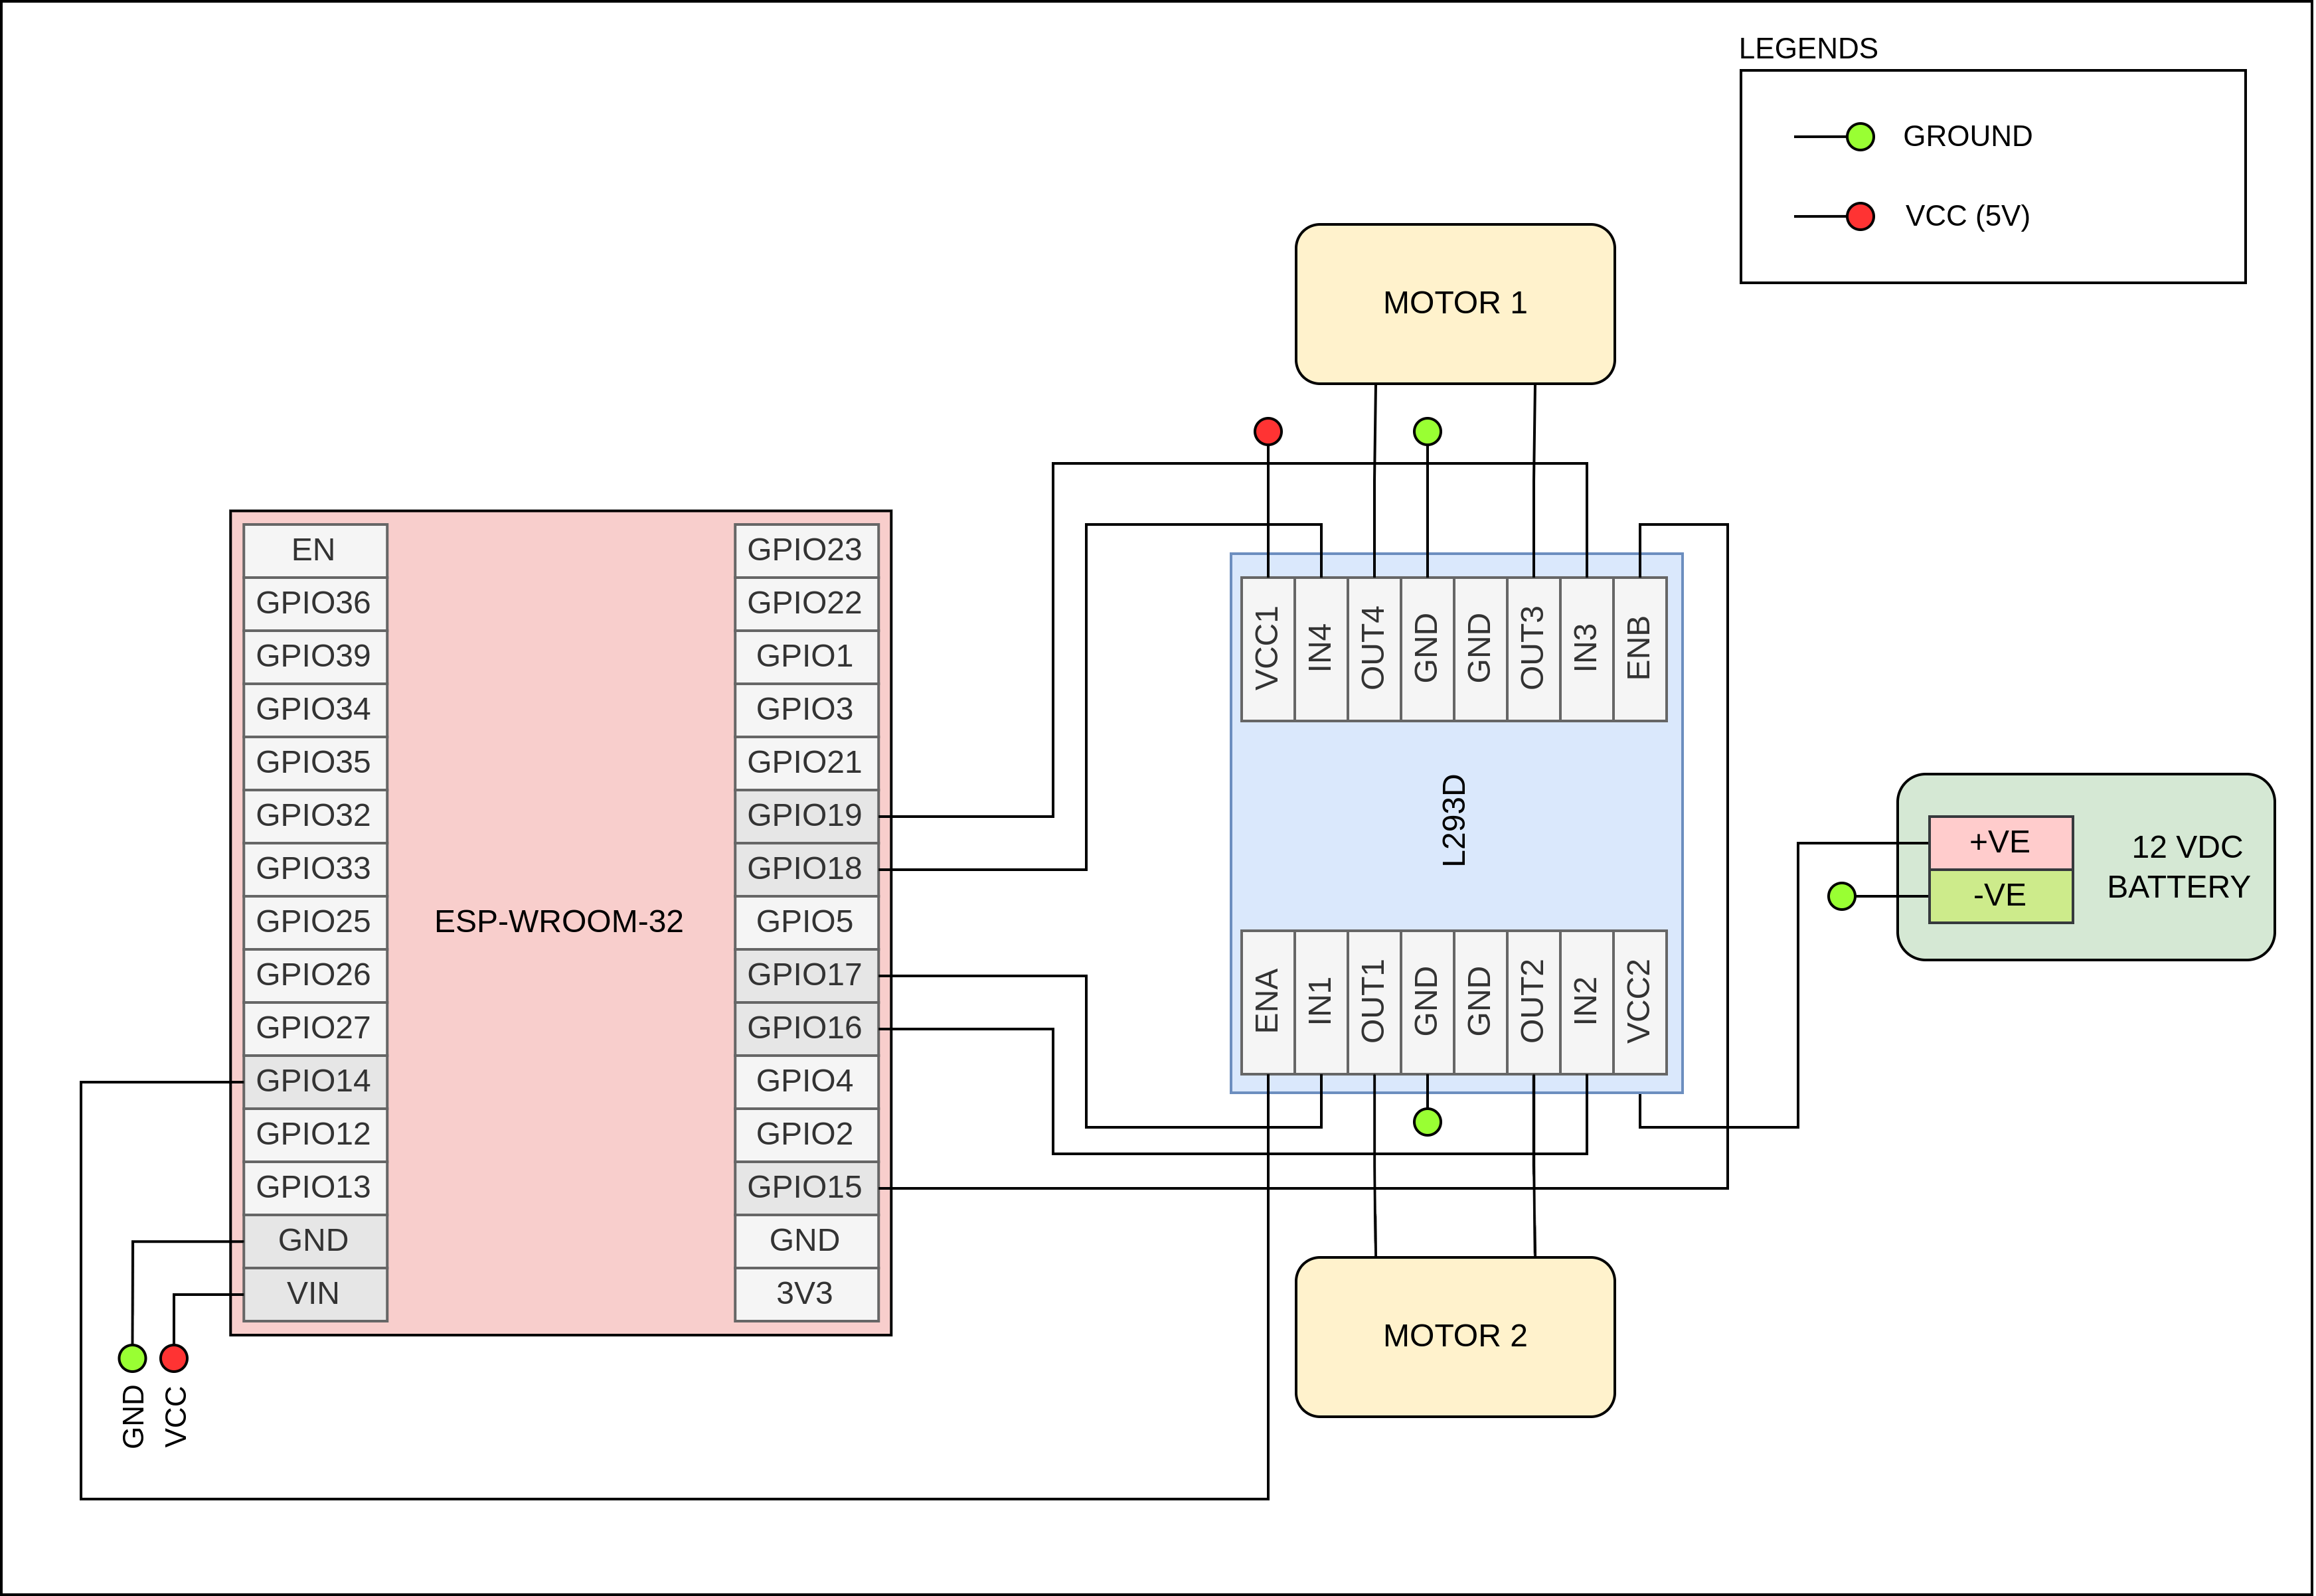
\includegraphics[width=0.6\columnwidth]{figs/beacon.png}
        \caption{Circuit Diagram for Beacon Tracking.}
        \label{fig:ckt}
    \end{figure}
\end{frame}

\section{Working}
\begin{frame}{Underlying Principles}
    \begin{enumerate}
        \item To estimate (radial) distance to beacon, we use its signal strength.
            For WiFi, this is the \textbf{Received Signal Strength Indicator} (RSSI).
        \pause
        \item The RSSI ($R$ dBm) at distance $d$ metres is given by
        \begin{align}
            R(d) = R(1) - 10\log_{10}\brak{d}
        \end{align}
        \pause
        \item Clearly, $R(d)$ is a convex function. Hence, we can use gradient 
        descent.
        \pause
        \item \textit{But how do we implement it?}
    \end{enumerate}
\end{frame}

\begin{frame}{Algorithm Description}
    Note that the following is a generic recursive description. For concrete 
    examples, please see slide number \autoref{software}.
    \pause
    \begin{enumerate}
        \item If the UGV is close enough to the beacon, terminate.
        \pause
        \item Take measurements at various points on a straight line.
        \pause
        \item Based on these measurements, decide the next move of the UGV, and 
        recurse till the UGV is close enough to the beacon.
    \end{enumerate}
\end{frame}

\section{Demonstration}
\begin{frame}
    \begin{center}
        \Huge In-Class Demonstration
    \end{center}
\end{frame}

\section{Conclusion}
\begin{frame}{Conclusions}
    \begin{enumerate}
        \item The UGV eventually converges close to the beacon.
        \pause
        \item However, if there are a lot of nearby obstacles, the UGV may not 
        converge close to the location of the beacon. It may either get physically 
        blocked by the beacon or the signal interference may be too high.
    \end{enumerate}
\end{frame}

\begin{frame}
    \begin{center}
        \Huge Thank You!
    \end{center}
\end{frame}
\end{document}
